\documentclass{beamer}

\usetheme{UiO}

\usepackage{array}
\usepackage{pgfplots}
\usepackage{pgfplotstable}

\usepgfplotslibrary{fillbetween}

\usetikzlibrary{arrows.meta}

\title{Exploring the brain with explainable artificial intelligence}
\subtitle{Characterizing diversity in patients with dementia}
\author{Esten H. Leonardsen}
\date{\today}

\begin{document}
	\begin{frame}
	 	\titlepage
	\end{frame}

    \newcommand{\mriside}[4]{
    \def\mridepth{0.75}

    \node[inner sep=0pt] (input) at (#1, #2) {
        \includegraphics[height=#3, width=#3]{#4}
    };

    \draw[fill=black] (input.north west) --
        ($ (input.north west) + (0.5 * \mridepth, 0.5 * \mridepth) $) --
        ($ (input.north east) + (0.5 * \mridepth, 0.5 * \mridepth) $) --
        (input.north east) -- cycle;
    \draw[fill=black] (input.north east) --
        ($ (input.north east) + (0.5 * \mridepth, 0.5 * \mridepth) $) --
        ($ (input.south east) + (0.5 * \mridepth, 0.5 * \mridepth) $) --
        (input.south east) -- cycle;
    \draw[] (input.north west) --
        ($ (input.north west) - (0.5 * \mridepth, 0.5 * \mridepth) $) --
        ($ (input.south west) - (0.5 * \mridepth, 0.5 * \mridepth) $) --
        (input.south west) -- cycle;
    \draw[] (input.north east) --
        ($ (input.north east) - (0.5 * \mridepth, 0.5 * \mridepth) $) --
        ($ (input.south east) - (0.5 * \mridepth, 0.5 * \mridepth) $) --
        (input.south east) -- cycle;
    \draw[] ($ (input.north west) - (0.5 * \mridepth, 0.5 * \mridepth) $) --
        ($ (input.north east) - (0.5 * \mridepth, 0.5 * \mridepth) $);
    \draw[] ($ (input.south west) - (0.5 * \mridepth, 0.5 * \mridepth) $) --
        ($ (input.south east) - (0.5 * \mridepth, 0.5 * \mridepth) $);
}


\newcommand{\inputside}[3]{
    \mriside{#1}{#2}{#3}{data/mri_sagittal.png}
}

\newcommand{\heatmapside}[3]{
    \mriside{#1}{#2}{#3}{data/combined_sagittal.png}
}

\newcommand{\convside}[6]{
    \def\sidex{#1}
    \def\sidey{#2}
    \def\sidewidth{#3}
    \def\sideheight{#4}
    \def\sidefillcolour{#5}
    \def\sidename{#6}

    \node[
        fill=\sidefillcolour,
        inner sep=0pt,
        outer sep=0pt,
        minimum width=\sidewidth,
        minimum height=\sideheight,
        draw=black
    ] (\sidename) at (\sidex, \sidey) {};
}

\newcommand{\convtop}[4]{
    \def\topbase{#1}
    \def\topwidth{#2}
    \def\topheight{#3}
    \def\topfillcolour{#4}

    \draw[fill=\topfillcolour,draw=black] #1 --
        ($ #1 + (#3, #3) $) --
        ($ #1 + (#3+#2, #3) $) --
        ($ #1 + (#2, 0) $);
}

\newcommand{\convfront}[3]{
    \def\frontbase{#1}
    \def\frontsize{#2}
    \def\frontfillcolour{#3}

    \draw[black, fill=\frontfillcolour] #1 --
        ($ #1 + (1*#2, 1*#2) $) --
        ($ #1 + (1*#2, 1*#2 - 2*#2) $) --
        ($ #1 + (0, -2*#2) $);
}

\newcommand{\convchannel}[7]{
    \def\channelx{#1}
    \def\channely{#2}
    \def\channelnodedepth{#3}
    \def\channelnodesize{#4}
    \def\channelnodecount{#5}
    \def\channelcolour{#6}
    \def\includefront{#7}

    \def\huemin{20}
    \def\huemax{80}

    \pgfmathsetmacro{\iterations}{#5-1}
    \foreach \i in {0,...,\iterations} {
        \pgfmathsetmacro{\hue}{int(random(\huemin, \huemax))}
        \convside{#1}{#2+\i*-#4}{#3 cm}{#4 cm}{#6!\hue}{n\i0}

        \foreach \j in {0,...,\iterations} {
            \pgfmathsetmacro{\innerhue}{int(random(\huemin, \huemax))}
            \ifnum\j=0
                \pgfmathsetmacro{\innerhue}{\hue}
            \fi

            \ifnum\includefront=1
                \convfront{($ (n00.north east) + (0.5*\j*#4, 0.5*\j*#4 - \i*#4) $)}{0.5*#4}{#6!\innerhue}
            \fi

            \ifnum\i=0
                \convtop{($ (n\i0.north west) + (0.5*\j*#4, 0.5*\j*#4) $)}{#3}{0.5*#4}{#6!\innerhue}
            \fi
        }
    }
}
\newcommand{\lrpchannel}[6]{
    \def\channelx{#1}
    \def\channely{#2}
    \def\channelnodedepth{#3}
    \def\channelnodesize{#4}
    \def\channelnodecount{#5}
    \def\includefront{#6}

    \colorlet{bgcolour}{black!85}

    \pgfmathsetmacro{\iterations}{#5-1}
    \foreach \i in {0,...,\iterations} {
        \pgfmathsetmacro{\hue}{int(random(-150, 100))}
        \colorlet{fillcolour}{bgcolour}

        \colorlet{lrpcolour}{red}
        \pgfmathsetmacro{\coinflip}{int(random(0, 1))}

        \ifnum\coinflip=1
            \colorlet{lrpcolour}{blue}
        \fi

        \ifnum\hue>0
            \colorlet{fillcolour}{lrpcolour!\hue!bgcolour}
        \fi

        \convside{#1}{#2+\i*-#4}{#3 cm}{#4 cm}{fillcolour}{n\i0}

        \foreach \j in {0,...,\iterations} {
            \pgfmathsetmacro{\innerhue}{int(random(-150, 100))}
            \colorlet{innerfillcolour}{bgcolour}

            \ifnum\innerhue>0
                \colorlet{innerfillcolour}{lrpcolour!\innerhue!bgcolour}
            \fi

            \ifnum\j=0
                \colorlet{innerfillcolour}{fillcolour}
            \fi

            \ifnum\includefront=1
                \convfront{($ (n00.north east) + (0.5*\j*#4, 0.5*\j*#4 - \i*#4) $)}{0.5*#4}{innerfillcolour}
            \fi

            \ifnum\i=0
                \convtop{($ (n\i0.north west) + (0.5*\j*#4, 0.5*\j*#4) $)}{#3}{0.5*#4}{innerfillcolour}
            \fi
        }
    }
}


\newcommand{\convlayer}[7]{
    \def\layerx{#1}
    \def\layery{#2}
    \def\layernodedepth{#3}
    \def\layernodesize{#4}
    \def\layernodecount{#5}
    \def\layerdepth{#6}
    \def\layercolour{#7}

    \pgfmathsetmacro{\layeriterations}{\layerdepth-1}
    \foreach \i in {0,...,\layeriterations}{
        \pgfmathsetmacro{\x}{\layerx + \i * \layernodedepth}
        \pgfmathsetmacro{\islast}{\i == \layeriterations ? 1 : 0}
        \convchannel{\x}{\layery}{\layernodedepth}{\layernodesize}{\layernodecount}{\layercolour}{\islast}
    }
}
\newcommand{\lrplayer}[6]{
    \def\layerx{#1}
    \def\layery{#2}
    \def\layernodedepth{#3}
    \def\layernodesize{#4}
    \def\layernodecount{#5}
    \def\layerdepth{#6}

    \pgfmathsetmacro{\layeriterations}{\layerdepth-1}
    \foreach \i in {0,...,\layeriterations}{
        \pgfmathsetmacro{\x}{\layerx + \i * \layernodedepth}
        \pgfmathsetmacro{\islast}{\i == \layeriterations ? 1 : 0}
        \lrpchannel{\x}{\layery}{\layernodedepth}{\layernodesize}{\layernodecount}{\islast}
    }
}

\newcommand{\modelarrow}[5]{
    \begin{scope}[transparency group, opacity=0.5]
        \draw[-stealth, line width=2pt, #3] #1 to [in=#4, out=#5] #2;
    \end{scope}
}
\newcommand{\cnnarrow}[3]{
    \modelarrow{#1}{#2}{#3}{180}{0}
}
\newcommand{\lrparrow}[3]{
    \modelarrow{#1}{#2}{#3}{0}{180}
}

\newcommand{\cnn}[6]{
    \def\xmin{#1}
    \def\ymin{#2}
    \def\nodedepth{#3}
    \def\nodesize{#4}
    \def\modelcolour{#5}
    \def\annotate{#6}

    \convlayer{#1 - 0.06 + 0.4}{#2 + 2.5 * #4}{#3}{#4}{12}{3}{\modelcolour}
    \cnnarrow{(#1 + 1.04, #2)}{(#1+2.2, #2)}{black}

    \convlayer{#1 + 1.44 + 0.4}{#2 + 1.5 * #4}{#3}{#4}{8}{5}{\modelcolour}
    \cnnarrow{(#1 + 2.59, #2)}{(#1+3.5, #2)}{black}

    \convlayer{#1 + 2.77 + 0.4}{#2 + 0.5 * #4}{#3}{#4}{4}{7}{\modelcolour}
    \cnnarrow{(#1 + 3.98, #2)}{(#1+5, #2)}{black}

    \convlayer{#1 + 3.93 + 0.4}{#2 + 0}{#3}{#4}{2}{9}{\modelcolour}

    \draw[thick, dashed] (#1 + 0.22, #2 + 1.43) --
                        (#1 + 5.4, #2 + 1.43) --
                        (#1 + 5.4, #2 - 1.42) --
                        (#1 + 0.22, #2 - 1.42) -- cycle;
    \node[anchor=south, text depth=0, font=\footnotesize\selectfont] at (#1 + 2.675, #2 + 1.43) {
        \textbf{Convolutional neural network}
    };
}
\newcommand{\lrp}[4]{
    \def\xmin{#1}
    \def\ymin{#2}
    \def\nodedepth{#3}
    \def\nodesize{#4}

    \lrplayer{#1 - 0.06 + 0.4}{#2 + 2.5 * #4}{#3}{#4}{12}{3}{black}
    \lrparrow{(#1+2.2, #2)}{(#1 + 1.04, #2)}{black}

    \lrplayer{#1 + 1.44 + 0.4}{#2 + 1.5 * #4}{#3}{#4}{8}{5}{black}
    \lrparrow{(#1+3.5, #2)}{(#1 + 2.59, #2)}{black}

    \lrplayer{#1 + 2.77 + 0.4}{#2 + 0.5 * #4}{#3}{#4}{4}{7}{black}
    \lrparrow{(#1+5, #2)}{(#1 + 3.98, #2)}{black}

    \lrplayer{#1 + 3.93 + 0.4}{#2 + 0}{#3}{#4}{2}{9}{black}

    \draw[thick, dashed] (#1 + 0.22, #2 + 1.43) --
                        (#1 + 5.4, #2 + 1.43) --
                        (#1 + 5.4, #2 - 1.42) --
                        (#1 + 0.22, #2 - 1.42) -- cycle;
    \node[anchor=south, text depth=0, font=\footnotesize\selectfont] at (#1 + 2.675, #2 + 1.43) {
        \textbf{Convolutional Neural Network}
    };
}

    % \begin{frame}{Dementia}
    %     \begin{tikzpicture}
    %         \node[] at (-5.25, -3.5) {};
    %         \node[] at (5.25, 3.5) {};

    %         \only<1>{
    %             \node[] at (0, 0) {
    %                 Dementia clinical
    %             };
    %         }
    %         \only<2>{
    %             \node[] at (0, 0) {
    %                 Dementia neuroimaging
    %             };
    %         }
    %         \only<3>{
    %             \node[] at (0, 0) {
    %                 Dementia prevalence
    %             };
    %         }
    %         \only<4>{
    %             \node[] at (0, 0) {
    %                 Dementia heterogeneity
    %             };
    %         }
    %     \end{tikzpicture}
    % \end{frame}

    
\newcommand{\mris}[1]{
    \begin{tikzpicture}
        \mriside{0.1}{0}{0.75cm}{0.375}{data/sagittal/0.png}
        \mriside{1.6}{0.1}{0.75cm}{0.375}{data/sagittal/1.png}
        \mriside{3.1}{-0.5}{0.75cm}{0.375}{data/sagittal/2.png}
        \mriside{1.5}{-1.3}{0.75cm}{0.375}{data/sagittal/3.png}
        \mriside{-0.1}{-1.2}{0.75cm}{0.375}{data/sagittal/4.png}

        \mriside{-0.1}{-3.25}{0.75cm}{0.375}{data/sagittal/5.png}
        \mriside{1.35}{-3.4}{0.75cm}{0.375}{data/sagittal/6.png}
        \mriside{3.1}{-3.1}{0.75cm}{0.375}{data/sagittal/7.png}
        \mriside{0.6}{-4.65}{0.75cm}{0.375}{data/sagittal/8.png}
        \mriside{2.3}{-4.7}{0.75cm}{0.375}{data/sagittal/9.png}

        \ifnum#1=1
            \node[font=\footnotesize, text=controls-default] at (1.6, 1) {
                Healthy controls (n=854)
            };
            \node[font=\footnotesize, text=cases-default] at (1.6, -5.6) {
                Dementia patients (n=854)
            };

            \draw[controls-default, dashed] (-0.85, 0.72)
                -- (3.85, 0.72)
                -- (3.85, -1.92)
                -- (-0.85, -1.92)
                -- cycle;
            \draw[cases-default, dashed] (-0.85, -2.48)
                -- (3.85, -2.48)
                -- (3.85, -5.32)
                -- (-0.85, -5.32)
                -- cycle;
        \fi
    \end{tikzpicture}
}

\newcommand{\dataset}{
    \def\legendfont{\footnotesize}

    \begin{tikzpicture}
        \begin{axis}[
            width=0.6\textwidth,
            height=0.8\textwidth,
            xmin=46,
            xmax=99,
            ymin=-1.6,
            ymax=1.2,
            xtick={60,70,80,90},
            axis lines=center,
            axis y line=none,
            clip=false,
            ticklabel style={font=\legendfont}
        ]
            \addplot[name path=zero, draw=none] coordinates {(47,0) (97,0)};

            \addplot[
                name path=fcases,
                draw=cases-default,
                very thick
            ] table [
                col sep=comma,
                x=x,
                y=F-cases
            ]{data/dementia_dataset/dementia_full.csv};\label{trace:cases}
            \addplot[fill=cases-default, opacity=0.2] fill between [of=zero and fcases];

            \addplot[
                name path=fcontrols,
                draw=controls-default,
                very thick
            ] table [
                col sep=comma,
                x=x,
                y=F-controls
            ]{data/dementia_dataset/dementia_full.csv};\label{trace:controls}
            \addplot[fill=controls-default, opacity=0.2] fill between [of=zero and fcontrols];

            \addplot[
                name path=mcases,
                draw=cases-default,
                very thick
            ] table [
                col sep=comma,
                x=x,y
                expr=\thisrow{M-cases} * -1
            ]{data/dementia_dataset/dementia_full.csv};
            \addplot[fill=cases-default, opacity=0.2] fill between [of=zero and mcases];

            \addplot[
                name path=mcontrols,
                draw=controls-default,
                very thick
            ] table [
                col sep=comma,
                x=x,
                y expr=\thisrow{M-controls} * -1
            ]{data/dementia_dataset/dementia_full.csv};
            \addplot[fill=controls-default, opacity=0.2] fill between [of=zero and mcontrols];

            \node[anchor=south west, font=\legendfont] at (axis cs: 43, 0.02) {\textbf{FEMALE}};
            \node[anchor=north west, font=\legendfont] at (axis cs: 43, -0.02) {\textbf{MALE}};
            \node[anchor=south, font=\legendfont, align=center] (n) at (axis cs: 76, -1.2) {\textbf{n=1708}};
        \end{axis}
    \end{tikzpicture}
}

\newcommand{\dementiapredictions}{

    \newcommand{\ymin}{-0.35}
    \newcommand{\ymax}{1.05}

    \begin{tikzpicture}
        \begin{axis}[
            name=distributions,
            height=0.6\textwidth,
            width=9.58cm,
            xtick pos=bottom,
            ymajorticks=false,
            xmajorticks=false,
            xmin=0,
            xmax=1,
            ymin=\ymin,
            ymax=\ymax,
            axis line style={draw=none}
        ]
            \addplot[
                name path=controls,
                draw=controls-default,
                very thick
            ] table [
                col sep=comma,
                x=prediction,
                y=controls
            ]{data/test_distributions.csv};

            \addplot[
                name path=cases,
                draw=cases-default,
                very thick
            ] table [
                col sep=comma,
                x=prediction,
                y=cases
            ]{data/test_distributions.csv};
            \addplot[name path=zero, draw=black] coordinates {(0,0) (1,0)};
            \addplot[fill=controls-default, opacity=0.2] fill between [of=zero and controls];
            \addplot[fill=cases-default, opacity=0.2] fill between [of=zero and cases];
            \addplot[
                scatter/classes={
                    control={controls-default, draw=black, opacity=0.5},
                    case={cases-default, draw=black, opacity=0.5}
                },
                scatter,
                mark=*,
                only marks,
                point meta=explicit symbolic
            ] table [
                col sep=comma,
                y expr=\thisrow{y} * -0.15 - 0.1,
                meta=class,
            ] {data/test_predictions.csv};
        \end{axis}

        \node[anchor=south west] at ($ (distributions.south east) + (0,0.63) $) {\footnotesize{Controls}};
        \node[anchor=south west] at ($ (distributions.south east) + (0,0.12) $) {\footnotesize{Patients}};
    \end{tikzpicture}
}

\begin{frame}{Methodology}
    \begin{tikzpicture}
        \node[draw=black] at (-5.25, -3.5) {};
        \node[draw=black] at (5.25, 3.5) {};

        \only<1>{
            \node[] at (-2.8, 0) {
                \mris{0}
            };
        }
        \only<2-3>{
            \node[] at (-2.8, 0) {
                \mris{1}
            };
        }
        \only<2>{
            \node[] at (2.5, -0.15) {
                \dataset
            };
        }

        \only<3>{
            \node[draw=black, fill=gray, minimum height=2.2cm, minimum width=3.7cm] (model) at (3.2, 0) {};
            \node[minimum height=2.2cm, minimum width=3.7cm, opacity=0.15] at (3.2, 0) {
                
\includegraphics[height=2cm]{data/gears.png}
            };
            \node[align=center, minimum height=2.2cm, minimum width=3.7cm, font=\normalfont\linespread{0.9}\bfseries\selectfont, text=white] at (3.2, 0) {
                Machine learning\\model
            };

            \begin{scope}[transparency group, opacity=0.5]
                \draw[-stealth, line width=4pt] (-0.5, 1.65) to [out=0, in=180] ($ (model.west) + (0, 0.22) $);
                \draw[-stealth, line width=4pt] (-0.495, -1.595) to [out=0, in=180] ($ (model.west) - (0, 0.22) $);
            \end{scope}
        }
        \only<5-6>{
            \mriside{-4}{1.45}{1.5cm}{0.75}{data/sagittal/0.png}
            \cnnarrow{(input.east)}{($ (input.center) + (2.5, 0) $)}{black}
        }
        \only<5>{
            \node[anchor=west, font=\small\linespread{0.9}\selectfont, text width=2cm] (healthy) at (3.5, 1.85) {
                Healthy\\control
            };
            \node[anchor=west, text depth=0] (patient) at (3.5, 1.05) {
                Patient
            };

            \cnnarrow{(2.61, 1.45)}{(healthy.west)}{black}
            \cnnarrow{(2.61, 1.45)}{(patient.west)}{black}
        }
        \only<6>{
            \node[anchor=west, text=black!25, font=\small\linespread{0.9}\selectfont, text width=2cm] (healthy) at (3.5, 1.85) {
                Healthy\\control
            };
            \node[anchor=west, text depth=0, font=\small] (patient) at (3.5, 1.05) {
                Patient
            };

            \cnnarrow{(2.61, 1.45)}{(healthy.west)}{black!25}
            \cnnarrow{(2.61, 1.45)}{(patient.west)}{black}
            \node[font=\small\linespread{0.9}\selectfont, align=center, anchor=north] at (-4, 0.25) {
                Healthy\\control
            };
        }
        \only<4-6>{
            \pgfmathsetseed{42}
            \node[] at (0, 1.7) {
                \cnn{0}{0}{0.066}{0.15}{black}{0}{0}
            };
        }

        \only<7-9>{
            \mriside{-4}{1.45}{1.5cm}{0.75}{data/mri_sagittal.png}
            \cnnarrow{(input.east)}{($ (input.center) + (2.5, 0) $)}{black}
            \pgfmathsetseed{43}
            \node[] at (0, 1.7) {
                \cnn{0}{0}{0.066}{0.15}{black}{0}{0}
            };
        }
        \only<7>{
            \node[anchor=west, text width=3cm, font=\small\linespread{0.9}\selectfont] (prediction) at (3.3, 1.45) {
                Predicted\\probability\\of dementia
            };
            \cnnarrow{(2.61, 1.45)}{(prediction.west)}{black}
        }
        \only<8-10>{
            \node[minimum width=8cm, left color=controls-default, right color=cases-default, text=white, draw=black, font=\small\bfseries\selectfont, inner sep=2pt] at (0, -2.75) {Predicted probability of dementia};
            \node[anchor=north] at (-4, -3.02) {0};
            \node[anchor=north] at (0, -3.02) {0.5};
            \node[anchor=north] at (4, -3.02) {1};
        }
        \only<8-9>{
            \node[anchor=west, text width=3cm, font=\small\linespread{0.9}\selectfont] (prediction) at (3.3, 1.45) {
                0.92
            };
            \cnnarrow{(2.61, 1.45)}{(prediction.west)}{black}
            \draw[very thick] (3.36, -3.12) -- (3.36, -2.38);
        }
        \only<9>{
            \node[font=\small] at (-4, 0.1) {
                Patient
            };
            \node[circle, fill=cases-default, draw=black, minimum size=0.14cm, inner sep=0pt, opacity=0.75] at (3.36, -2.2) {};
        }
        \only<10>{
            \node[anchor=south] at (0.576, -2.65) {
                \dementiapredictions
            };
        }
    \end{tikzpicture}
\end{frame}

    % \newcommand{\neuron}[3]{
    \node[circle, draw=black, fill=#2] (#1) at #3 {};
}

\begin{frame}{Explainable artificial intelligence}
    \begin{tikzpicture}
        \node[] at (-5.25, -3.5) {};
        \node[] at (5.25, 3.5) {};

        \node[
            draw=black,
            fill=cyan!15,
            minimum height=3cm,
            minimum width=4.3cm,
            label=above:\footnotesize{\textbf{Artificial neural network}}
        ] (model) at (0, 0) {};

        \def\hsep{0.7}
        \def\vsep{0.5}
        \def\edgecolor{gray}
        \def\edgeopacity{0.5}
        \def\neuroncolour{gray}

        \only<1>{
            \neuron{n00}{\neuroncolour}{($ (model) + (-2 * \hsep, -2 * \vsep) $)}
            \neuron{n01}{\neuroncolour}{($ (model) + (-2 * \hsep, -\vsep) $)}
            \neuron{n02}{\neuroncolour}{($ (model) + (-2 * \hsep, 0) $)}
            \neuron{n03}{\neuroncolour}{($ (model) + (-2 * \hsep, \vsep) $)}
            \neuron{n04}{\neuroncolour}{($ (model) + (-2 * \hsep, 2 * \vsep) $)}

            \neuron{n10}{\neuroncolour}{($ (model) + (-\hsep, -1.5 * \vsep) $)}
            \neuron{n11}{\neuroncolour}{($ (model) + (-\hsep, -0.5 * \vsep) $)}
            \neuron{n12}{\neuroncolour}{($ (model) + (-\hsep, 0.5 * \vsep) $)}
            \neuron{n13}{\neuroncolour}{($ (model) + (-\hsep, 1.5 * \vsep) $)}

            \neuron{n20}{\neuroncolour}{($ (model) + (0, -\vsep) $)}
            \neuron{n21}{\neuroncolour}{(model)}
            \neuron{n22}{\neuroncolour}{($ (model) + (0, \vsep) $)}

            \neuron{n30}{\neuroncolour}{($ (model) + (\hsep, -0.5 * \vsep) $)}
            \neuron{n31}{\neuroncolour}{($ (model) + (\hsep, 0.5 * \vsep) $)}

            \neuron{n40}{\neuroncolour}{($ (model) + (2 * \hsep, 0) $)}

            \draw[-stealth, \edgecolor, opacity=\edgeopacity] (model.west) -- (n00);
            \draw[-stealth, \edgecolor, opacity=\edgeopacity] (model.west) -- (n01);
            \draw[-stealth, \edgecolor, opacity=\edgeopacity] (model.west) -- (n02);
            \draw[-stealth, \edgecolor, opacity=\edgeopacity] (model.west) -- (n03);
            \draw[-stealth, \edgecolor, opacity=\edgeopacity] (model.west) -- (n04);

            \foreach \i in {0,...,4} {
                \foreach \j in {0,...,3} {
                    \draw[\edgecolor, opacity=\edgeopacity] (n0\i) -- (n1\j);
                }
            }
            \foreach \i in {0,...,3} {
                \foreach \j in {0,...,2} {
                    \draw[\edgecolor, opacity=\edgeopacity] (n1\i) -- (n2\j);
                }
            }
            \foreach \i in {0,...,2} {
                \foreach \j in {0,...,1} {
                    \draw[\edgecolor, opacity=\edgeopacity] (n2\i) -- (n3\j);
                }
            }
            \foreach \i in {0,...,1} {
                \draw[\edgecolor, opacity=\edgeopacity] (n3\i) -- (n40);
            }

            \draw[-stealth, \edgecolor, opacity=\edgeopacity] (n40) -- (model.east);
        }
        \only<2>{
            \neuron{n00}{black!25}{($ (model) + (-2 * \hsep, -2 * \vsep) $)}
            \neuron{n01}{black!90}{($ (model) + (-2 * \hsep, -\vsep) $)}
            \neuron{n02}{black!72}{($ (model) + (-2 * \hsep, 0) $)}
            \neuron{n03}{black!99}{($ (model) + (-2 * \hsep, \vsep) $)}
            \neuron{n04}{black!10}{($ (model) + (-2 * \hsep, 2 * \vsep) $)}

            \neuron{n10}{black!55}{($ (model) + (-\hsep, -1.5 * \vsep) $)}
            \neuron{n11}{black!92}{($ (model) + (-\hsep, -0.5 * \vsep) $)}
            \neuron{n12}{black!31}{($ (model) + (-\hsep, 0.5 * \vsep) $)}
            \neuron{n13}{black!7}{($ (model) + (-\hsep, 1.5 * \vsep) $)}

            \neuron{n20}{black!50}{($ (model) + (0, -\vsep) $)}
            \neuron{n21}{black!10}{(model)}
            \neuron{n22}{black!100}{($ (model) + (0, \vsep) $)}

            \neuron{n30}{black!75}{($ (model) + (\hsep, -0.5 * \vsep) $)}
            \neuron{n31}{black!65}{($ (model) + (\hsep, 0.5 * \vsep) $)}

            \neuron{n40}{black!95}{($ (model) + (2 * \hsep, 0) $)}

            \draw[-stealth, \edgecolor, opacity=\edgeopacity] (model.west) -- (n00);
            \draw[-stealth, \edgecolor, opacity=\edgeopacity] (model.west) -- (n01);
            \draw[-stealth, \edgecolor, opacity=\edgeopacity] (model.west) -- (n02);
            \draw[-stealth, \edgecolor, opacity=\edgeopacity] (model.west) -- (n03);
            \draw[-stealth, \edgecolor, opacity=\edgeopacity] (model.west) -- (n04);

            \foreach \i in {0,...,4} {
                \foreach \j in {0,...,3} {
                    \draw[\edgecolor, opacity=\edgeopacity] (n0\i) -- (n1\j);
                }
            }
            \foreach \i in {0,...,3} {
                \foreach \j in {0,...,2} {
                    \draw[\edgecolor, opacity=\edgeopacity] (n1\i) -- (n2\j);
                }
            }
            \foreach \i in {0,...,2} {
                \foreach \j in {0,...,1} {
                    \draw[\edgecolor, opacity=\edgeopacity] (n2\i) -- (n3\j);
                }
            }
            \foreach \i in {0,...,1} {
                \draw[\edgecolor, opacity=\edgeopacity] (n3\i) -- (n40);
            }

            \draw[-stealth, \edgecolor, opacity=\edgeopacity] (n40) -- (model.east);

            \node[anchor=east, draw=black, inner sep=0pt] (input) at ($ (model.west) + (-0.77, 0) $) {
                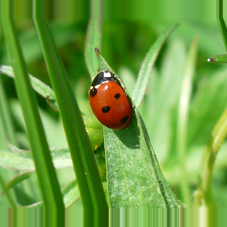
\includegraphics[width=2cm]{data/ladybug.png}
            };
            \cnnarrow{(input.east)}{(model.west)}{black}

            \node[anchor=west] (output) at ($ (model.east) + (0.77, 0) $) {
                Ladybug
            };
            \cnnarrow{(model.east)}{(output.west)}{black}

            \draw[-Latex, line width=3pt] ($ (model.south west) + (0.1, -0.4) $) -- ($ (model.south east) + (-0.1, -0.4) $);

            \node[] at (0, -2.3) {
                \textit{Forward pass}
            };
        }
        \only<3>{
            \neuron{n00}{red!25!black}{($ (model) + (-2 * \hsep, -2 * \vsep) $)}
            \neuron{n01}{red!90!black}{($ (model) + (-2 * \hsep, -\vsep) $)}
            \neuron{n02}{yellow!15!red}{($ (model) + (-2 * \hsep, 0) $)}
            \neuron{n03}{red!99!black}{($ (model) + (-2 * \hsep, \vsep) $)}
            \neuron{n04}{red!10!black}{($ (model) + (-2 * \hsep, 2 * \vsep) $)}

            \neuron{n10}{red!55!black}{($ (model) + (-\hsep, -1.5 * \vsep) $)}
            \neuron{n11}{yellow!20!red}{($ (model) + (-\hsep, -0.5 * \vsep) $)}
            \neuron{n12}{yellow!90!red}{($ (model) + (-\hsep, 0.5 * \vsep) $)}
            \neuron{n13}{red!7!black}{($ (model) + (-\hsep, 1.5 * \vsep) $)}

            \neuron{n20}{red!90!black}{($ (model) + (0, -\vsep) $)}
            \neuron{n21}{red!30!black}{(model)}
            \neuron{n22}{yellow!70!red}{($ (model) + (0, \vsep) $)}

            \neuron{n30}{yellow!40!red}{($ (model) + (\hsep, -0.5 * \vsep) $)}
            \neuron{n31}{red!65!black}{($ (model) + (\hsep, 0.5 * \vsep) $)}

            \neuron{n40}{red}{($ (model) + (2 * \hsep, 0) $)}

            \draw[stealth-, red, opacity=\edgeopacity] (model.west) -- (n00);
            \draw[stealth-, red, opacity=\edgeopacity] (model.west) -- (n01);
            \draw[stealth-, red, opacity=\edgeopacity] (model.west) -- (n02);
            \draw[stealth-, red, opacity=\edgeopacity] (model.west) -- (n03);
            \draw[stealth-, red, opacity=\edgeopacity] (model.west) -- (n04);

            \foreach \i in {0,...,4} {
                \foreach \j in {0,...,3} {
                    \draw[red, opacity=\edgeopacity] (n0\i) -- (n1\j);
                }
            }
            \foreach \i in {0,...,3} {
                \foreach \j in {0,...,2} {
                    \draw[red, opacity=\edgeopacity] (n1\i) -- (n2\j);
                }
            }
            \foreach \i in {0,...,2} {
                \foreach \j in {0,...,1} {
                    \draw[red, opacity=\edgeopacity] (n2\i) -- (n3\j);
                }
            }
            \foreach \i in {0,...,1} {
                \draw[red, opacity=\edgeopacity] (n3\i) -- (n40);
            }

            \draw[stealth-, red, opacity=\edgeopacity] (n40) -- (model.east);

            \node[anchor=east, draw=black, inner sep=0pt] (input) at ($ (model.west) + (-0.77, 0) $) {
                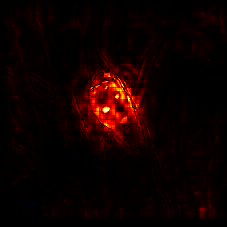
\includegraphics[width=2cm]{data/ladybug_explanation.png}
            };
            \lrparrow{(model.west)}{(input.east)}{red}

            \node[anchor=west, text=red] (output) at ($ (model.east) + (0.77, 0) $) {
                Ladybug
            };
            \lrparrow{(output.west)}{(model.east)}{red}

            \draw[Latex-, line width=3pt, red] ($ (model.south west) + (0.1, -0.4) $) -- ($ (model.south east) + (-0.1, -0.4) $);

            \node[text=red] at (0, -2.3) {
                \textit{Backward pass}
            };
        }
    \end{tikzpicture}
\end{frame}


    % \begin{frame}{Explainable AI and dementia}
    %     \begin{tikzpicture}
    %         \node[] at (-5.25, -3.5) {};
    %         \node[] at (5.25, 3.5) {};

    %         \only<1>{
    %             \mriside{-4}{-0.25}{1.5cm}{0.75}{data/mri_sagittal.png}
    %             \cnnarrow{(input.east)}{($ (input.center) + (2.5, 0) $)}{black}
    %             \pgfmathsetseed{43}
    %             \node[] at (0, 0) {
    %                 \cnn{0}{0}{0.066}{0.15}{black}{0}{0}
    %             };
    %             \node[anchor=west, text width=3cm, font=\small\linespread{0.9}\selectfont] (prediction) at (3.3, -0.25) {
    %                 0.92
    %             };
    %             \cnnarrow{(2.61, -0.25)}{(prediction.west)}{black}
    %         }

    %         \only<2>{
    %             \mriside{-4}{-0.25}{1.5cm}{0.75}{data/combined_sagittal.png}
    %             \lrparrow{($ (input.center) + (2.5, 0) $)}{(input.east)}{red}
    %             \pgfmathsetseed{43}
    %             \node[] at (0.16, 0) {
    %                 \lrp{0}{0}{0.066}{0.15}
    %             };
    %             \node[anchor=west, text width=3cm, font=\small\linespread{0.9}\selectfont] (prediction) at (3.3, -0.25) {
    %                 0.92
    %             };
    %             \lrparrow{(prediction.west)}{(2.61, -0.25)}{red}
    %         }

    %         \only<3>{
    %             \node[
    %                 minimum height=0.41\textwidth,
    %                 minimum width=0.32\textwidth,
    %                 fill=black,
    %                 anchor=west
    %             ] (box1) at (-5.25, 0) {};
    %             \node[anchor=south] at (box1.south) {
    %                 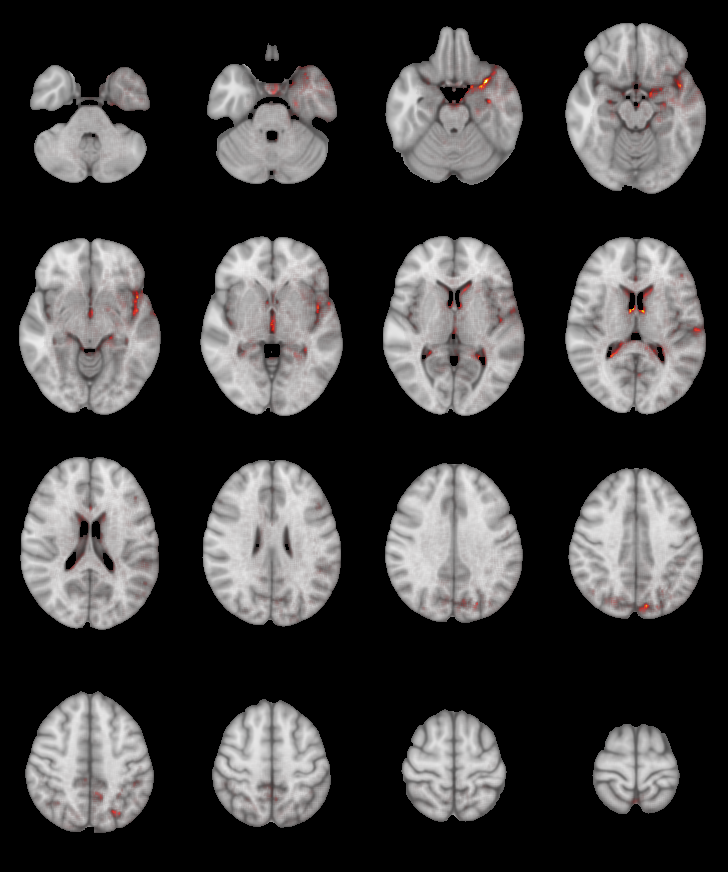
\includegraphics[width=0.31\textwidth]{data/subject1.png}
    %             };
    %             \node[anchor=north,inner sep=2pt, text=white, font=\footnotesize] at (box1.north) {Patient 1};

    %             \node
    %                 [minimum height=0.41\textwidth,
    %                 minimum width=0.32\textwidth,
    %                 fill=black,
    %                 anchor=west
    %             ] (box2) at ($ (box1.east) + (0.05,0) $) {};
    %             \node[anchor=south] at (box2.south) {
    %                 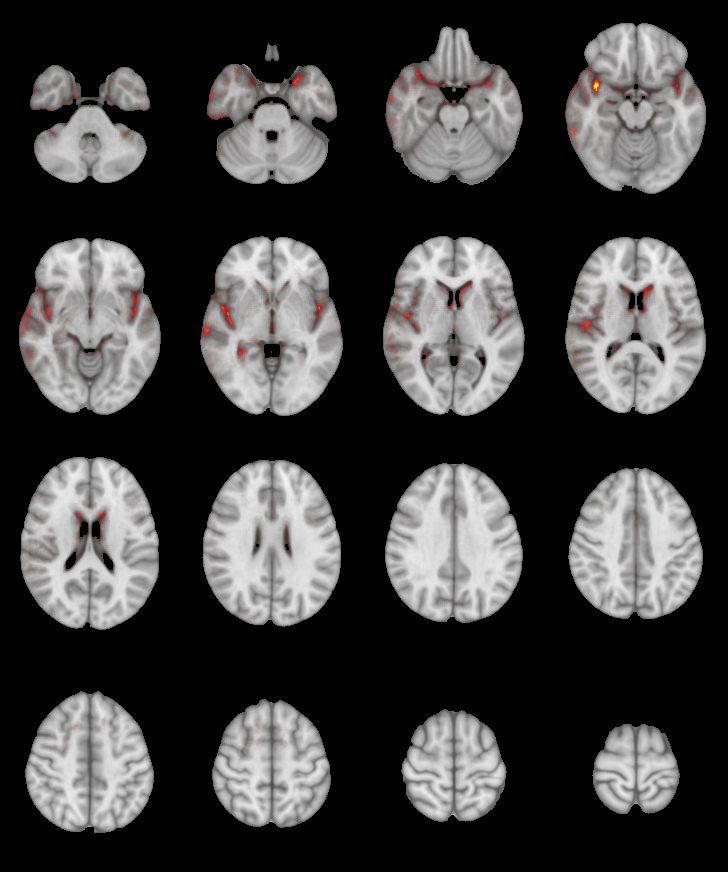
\includegraphics[width=0.31\textwidth]{data/subject2.png}
    %             };
    %             \node[anchor=north,inner sep=3pt, text=white, font=\footnotesize] at (box2.north) {Partient 2};

    %             \node
    %                 [minimum height=0.41\textwidth,
    %                 minimum width=0.32\textwidth,
    %                 fill=black,
    %                 anchor=west
    %             ] (box3) at ($ (box2.east) + (0.05,0) $) {};
    %             \node[anchor=south] at (box3.south) {
    %                 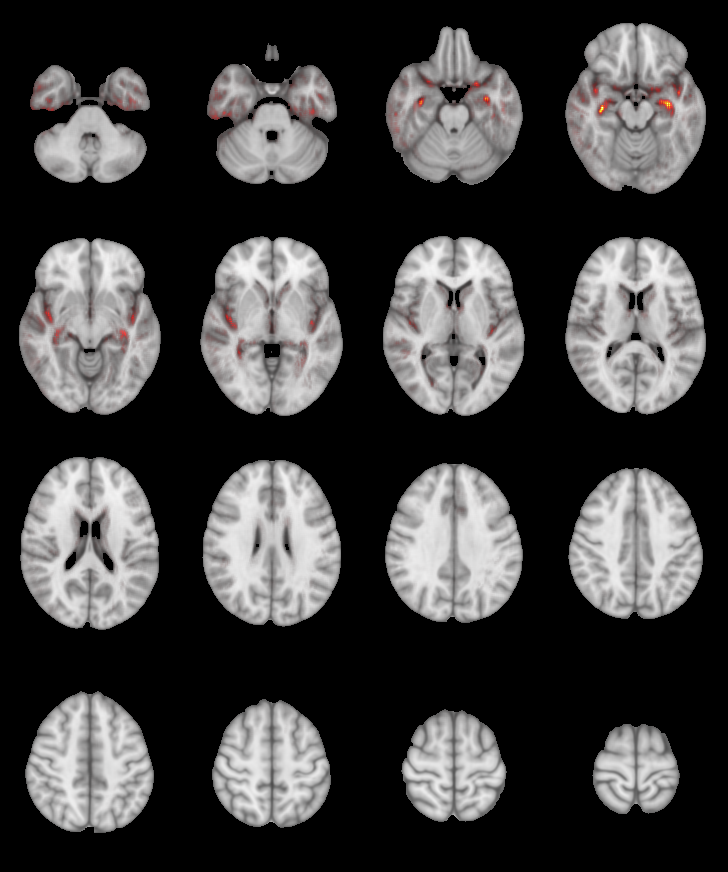
\includegraphics[width=0.31\textwidth]{data/subject3.png}
    %             };
    %             \node[anchor=north,inner sep=3pt, text=white, font=\footnotesize] at (box3.north) {Patient 3};
    %         }
    %     \end{tikzpicture}
    % \end{frame}

    % 
\begin{frame}{Explainable AI: Caveats}
    \begin{tikzpicture}
        \node[] at (-5.25, -3.5) {};
        \node[] at (5.25, 3.5) {};

        \node[
            draw=black,
            fill=cyan!15,
            minimum height=3cm,
            minimum width=4.3cm,
            label=above:\footnotesize{\textbf{Artificial neural network}}
        ] (model) at (0, 0) {};

        \def\hsep{0.7}
        \def\vsep{0.5}
        \def\edgecolor{gray}
        \def\edgeopacity{0.5}
        \def\neuroncolour{gray}

        \only<1>{
            \neuron{n00}{black!25}{($ (model) + (-2 * \hsep, -2 * \vsep) $)}
            \neuron{n01}{black!90}{($ (model) + (-2 * \hsep, -\vsep) $)}
            \neuron{n02}{black!72}{($ (model) + (-2 * \hsep, 0) $)}
            \neuron{n03}{black!99}{($ (model) + (-2 * \hsep, \vsep) $)}
            \neuron{n04}{black!10}{($ (model) + (-2 * \hsep, 2 * \vsep) $)}

            \neuron{n10}{black!55}{($ (model) + (-\hsep, -1.5 * \vsep) $)}
            \neuron{n11}{black!92}{($ (model) + (-\hsep, -0.5 * \vsep) $)}
            \neuron{n12}{black!31}{($ (model) + (-\hsep, 0.5 * \vsep) $)}
            \neuron{n13}{black!7}{($ (model) + (-\hsep, 1.5 * \vsep) $)}

            \neuron{n20}{black!50}{($ (model) + (0, -\vsep) $)}
            \neuron{n21}{black!10}{(model)}
            \neuron{n22}{black!100}{($ (model) + (0, \vsep) $)}

            \neuron{n30}{black!75}{($ (model) + (\hsep, -0.5 * \vsep) $)}
            \neuron{n31}{black!65}{($ (model) + (\hsep, 0.5 * \vsep) $)}

            \neuron{n40}{black!95}{($ (model) + (2 * \hsep, 0) $)}

            \draw[-stealth, \edgecolor, opacity=\edgeopacity] (model.west) -- (n00);
            \draw[-stealth, \edgecolor, opacity=\edgeopacity] (model.west) -- (n01);
            \draw[-stealth, \edgecolor, opacity=\edgeopacity] (model.west) -- (n02);
            \draw[-stealth, \edgecolor, opacity=\edgeopacity] (model.west) -- (n03);
            \draw[-stealth, \edgecolor, opacity=\edgeopacity] (model.west) -- (n04);

            \foreach \i in {0,...,4} {
                \foreach \j in {0,...,3} {
                    \draw[\edgecolor, opacity=\edgeopacity] (n0\i) -- (n1\j);
                }
            }
            \foreach \i in {0,...,3} {
                \foreach \j in {0,...,2} {
                    \draw[\edgecolor, opacity=\edgeopacity] (n1\i) -- (n2\j);
                }
            }
            \foreach \i in {0,...,2} {
                \foreach \j in {0,...,1} {
                    \draw[\edgecolor, opacity=\edgeopacity] (n2\i) -- (n3\j);
                }
            }
            \foreach \i in {0,...,1} {
                \draw[\edgecolor, opacity=\edgeopacity] (n3\i) -- (n40);
            }

            \draw[-stealth, \edgecolor, opacity=\edgeopacity] (n40) -- (model.east);

            \node[anchor=east, draw=black, inner sep=0pt] (input) at ($ (model.west) + (-0.77, 0) $) {
                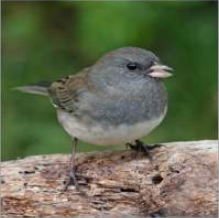
\includegraphics[width=2cm]{data/bird.png}
            };
            \cnnarrow{(input.east)}{(model.west)}{black}

            \node[anchor=west] (output) at ($ (model.east) + (0.77, 0) $) {
                Bird
            };
            \cnnarrow{(model.east)}{(output.west)}{black}
        }
        \only<2>{
            \neuron{n00}{red!25!black}{($ (model) + (-2 * \hsep, -2 * \vsep) $)}
            \neuron{n01}{red!90!black}{($ (model) + (-2 * \hsep, -\vsep) $)}
            \neuron{n02}{yellow!15!red}{($ (model) + (-2 * \hsep, 0) $)}
            \neuron{n03}{red!99!black}{($ (model) + (-2 * \hsep, \vsep) $)}
            \neuron{n04}{red!10!black}{($ (model) + (-2 * \hsep, 2 * \vsep) $)}

            \neuron{n10}{red!55!black}{($ (model) + (-\hsep, -1.5 * \vsep) $)}
            \neuron{n11}{yellow!20!red}{($ (model) + (-\hsep, -0.5 * \vsep) $)}
            \neuron{n12}{yellow!90!red}{($ (model) + (-\hsep, 0.5 * \vsep) $)}
            \neuron{n13}{red!7!black}{($ (model) + (-\hsep, 1.5 * \vsep) $)}

            \neuron{n20}{red!90!black}{($ (model) + (0, -\vsep) $)}
            \neuron{n21}{red!30!black}{(model)}
            \neuron{n22}{yellow!70!red}{($ (model) + (0, \vsep) $)}

            \neuron{n30}{yellow!40!red}{($ (model) + (\hsep, -0.5 * \vsep) $)}
            \neuron{n31}{red!65!black}{($ (model) + (\hsep, 0.5 * \vsep) $)}

            \neuron{n40}{red}{($ (model) + (2 * \hsep, 0) $)}

            \draw[stealth-, red, opacity=\edgeopacity] (model.west) -- (n00);
            \draw[stealth-, red, opacity=\edgeopacity] (model.west) -- (n01);
            \draw[stealth-, red, opacity=\edgeopacity] (model.west) -- (n02);
            \draw[stealth-, red, opacity=\edgeopacity] (model.west) -- (n03);
            \draw[stealth-, red, opacity=\edgeopacity] (model.west) -- (n04);

            \foreach \i in {0,...,4} {
                \foreach \j in {0,...,3} {
                    \draw[red, opacity=\edgeopacity] (n0\i) -- (n1\j);
                }
            }
            \foreach \i in {0,...,3} {
                \foreach \j in {0,...,2} {
                    \draw[red, opacity=\edgeopacity] (n1\i) -- (n2\j);
                }
            }
            \foreach \i in {0,...,2} {
                \foreach \j in {0,...,1} {
                    \draw[red, opacity=\edgeopacity] (n2\i) -- (n3\j);
                }
            }
            \foreach \i in {0,...,1} {
                \draw[red, opacity=\edgeopacity] (n3\i) -- (n40);
            }

            \draw[stealth-, red, opacity=\edgeopacity] (n40) -- (model.east);

            \node[anchor=east, draw=black, inner sep=0pt] (input) at ($ (model.west) + (-0.77, 0) $) {
                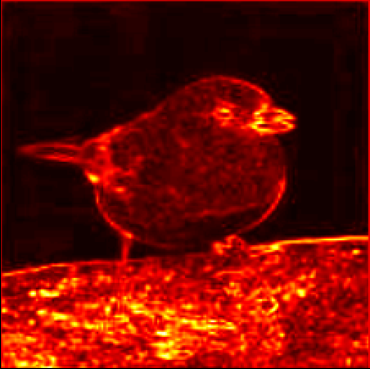
\includegraphics[width=2cm]{data/edgedetector.png}
            };
            \lrparrow{(model.west)}{(input.east)}{red}

            \node[anchor=west, text=red] (output) at ($ (model.east) + (0.77, 0) $) {
                Bird
            };
            \lrparrow{(output.west)}{(model.east)}{red}
        }
    \end{tikzpicture}
\end{frame}

    % \newcommand{\mriwidth}{2.2cm}
\newcommand{\gap}{0.00cm}

\newcommand{\correlationplot}[4]{
    \definecolor{color0}{rgb}{0.62, 0.004, 0.259}
    \definecolor{color1}{rgb}{0.755, 0.154, 0.291}
    \definecolor{color2}{rgb}{0.866, 0.29, 0.298}
    \definecolor{color3}{rgb}{0.943, 0.406, 0.268}
    \definecolor{color4}{rgb}{0.975, 0.557, 0.323}
    \definecolor{color5}{rgb}{0.993, 0.709, 0.403}
    \definecolor{color6}{rgb}{0.995, 0.832, 0.506}
    \definecolor{color7}{rgb}{0.998, 0.926, 0.625}
    \definecolor{color8}{rgb}{0.998, 0.999, 0.746}
    \definecolor{color9}{rgb}{0.937, 0.975, 0.65}
    \definecolor{color10}{rgb}{0.838, 0.935, 0.609}
    \definecolor{color11}{rgb}{0.693, 0.876, 0.639}
    \definecolor{color12}{rgb}{0.527, 0.811, 0.645}
    \definecolor{color13}{rgb}{0.368, 0.725, 0.662}
    \definecolor{color14}{rgb}{0.24, 0.582, 0.721}
    \definecolor{color15}{rgb}{0.267, 0.441, 0.698}
    \definecolor{color16}{rgb}{0.369, 0.31, 0.635}

    \begin{tikzpicture}
        \begin{axis}[
            height=1.715 * \mriwidth,
            width=1.715 * \mriwidth,
            xmajorticks=false,
            ylabel=#3,
            ytick={0, 2, 4, 6, 8},
            yticklabels=#2,
            xmin=-1,
            xmax=17,
            ymin=0,
            ymax=9,
            every tick label/.append style={font=\tiny},
            ytick pos=left,
            scatter/classes={
                ADNI_EF={color0, draw=black},
                ADNI_MEM={color1, draw=black},
                CDCARE={color2, draw=black},
                CDCOMMUN={color3, draw=black},
                CDGLOBAL={color4, draw=black},
                CDHOME={color5, draw=black},
                CDJUDGE={color6, draw=black},
                CDMEMORY={color7, draw=black},
                CDORIENT={color8, draw=black},
                FAQTOTAL={color9, draw=black},
                GDTOTAL={color10, draw=black},
                MMSCORE={color11, draw=black},
                NPISCORE={color12, draw=black},
                PHC_EXF={color13, draw=black},
                PHC_LAN={color14, draw=black},
                PHC_MEM={color15, draw=black},
                PHC_VSP={color16, draw=black}
            },
            y label style={at={(-0.1,0.5)}},
            ymajorgrids=true,
            ytick style={draw=none},
            clip=false,
            grid style={draw=gray!20},
            axis line style={draw=gray!70}
        ]
            \addplot[
                only marks,
                scatter,
                scatter src=explicit symbolic
            ] table [
                col sep=comma,
                x=index,
                y=component_#1,
                meta=symptom
            ] {data/correlations.csv};
            \addplot[dashed,red, thick] coordinates {
                (-1, 2.76)
                (17, 2.76)
            };
            #4
        \end{axis}
    \end{tikzpicture}
}

\newsavebox{\firstcorrelations}
\sbox{\firstcorrelations}{%
    \correlationplot{0}{{0, 2, 4, 6, 8}}{\scriptsize{$-log_{10}(p)$}}{
        \node[] at (axis cs: 14, 6.19) {\tiny{PHC\_LAN}};
    }
}
\newsavebox{\secondcorrelations}
\sbox{\secondcorrelations}{%
    \correlationplot{1}{{,,}}{{}}{
        \node[] at (axis cs: 9, 3.74) {\tiny{FAQTOTAL}};
    }
}
\newsavebox{\thirdcorrelations}
\sbox{\thirdcorrelations}{%
    \correlationplot{2}{{,,}}{{}}{
        \node[] at (axis cs: 0, 6.44) {\tiny{ADNI\_EF}};
        \node[] at (axis cs: 13, 7.95) {\tiny{PHC\_EXF}};
    }
}
\newsavebox{\fourthcorrelations}
\sbox{\fourthcorrelations}{%
    \correlationplot{3}{{,,}}{{}}{
        \node[] at (axis cs: 0, 9.02) {\tiny{ADNI\_EF}};
        \node[] at (axis cs: 13, 8.75) {\tiny{PHC\_EXF}};
        \node[] at (axis cs: 14, 5.84) {\tiny{PHC\_LAN}};
        \node[] at (axis cs: 6, 5.18) {\tiny{CDJUDGE}};
        \node[] at (axis cs: 11, 3.99) {\tiny{MMSCORE}};
    }
}

\newcommand{\cognitivecorrelations}[1]{
    \begin{tikzpicture}
        \node[] at (-1.7, 1.2) {};
        \node[] at (8.7, -5) {};

        \node[] (first) at (0, 0) {
            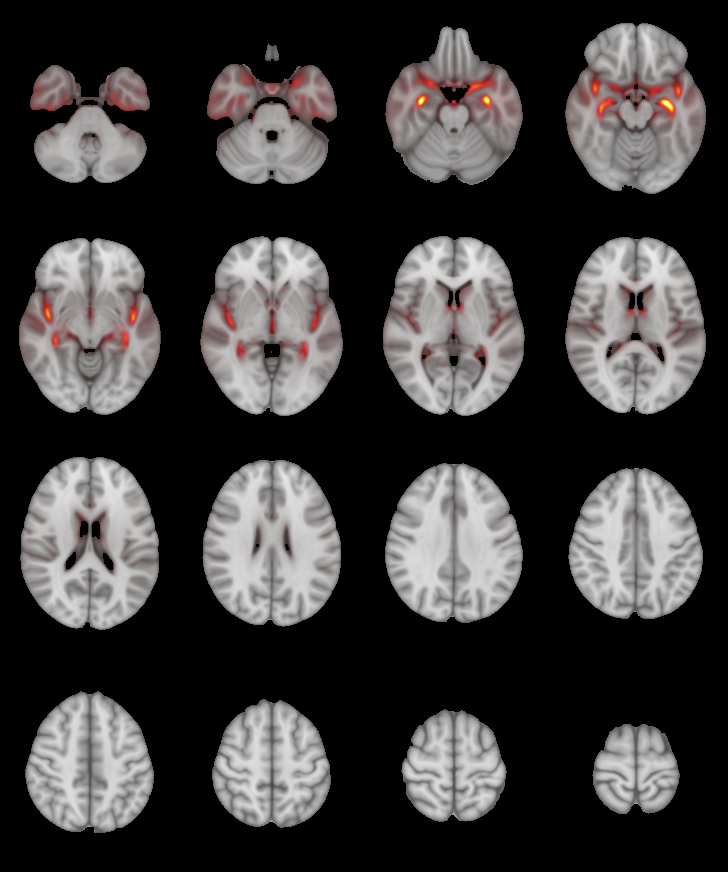
\includegraphics[
                width=\mriwidth,
                clip=true,
                trim = 192mm 232mm 0mm 0mm
            ]{data/components/component_0.png}
        };

        \node[anchor=west] (second) at ($ (first.east) + (\gap, 0) $) {
            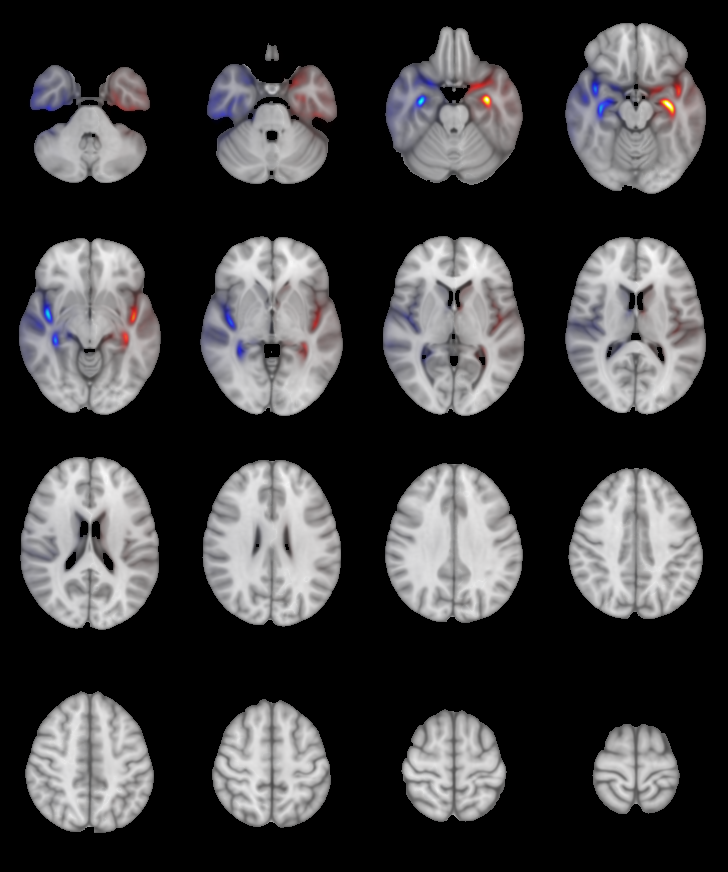
\includegraphics[
                width=\mriwidth,
                clip=true,
                trim = 192mm 232mm 0mm 0mm
            ]{data/components/component_1.png}
        };
        \node[anchor=west] (third) at ($ (second.east) + (\gap, 0) $) {
            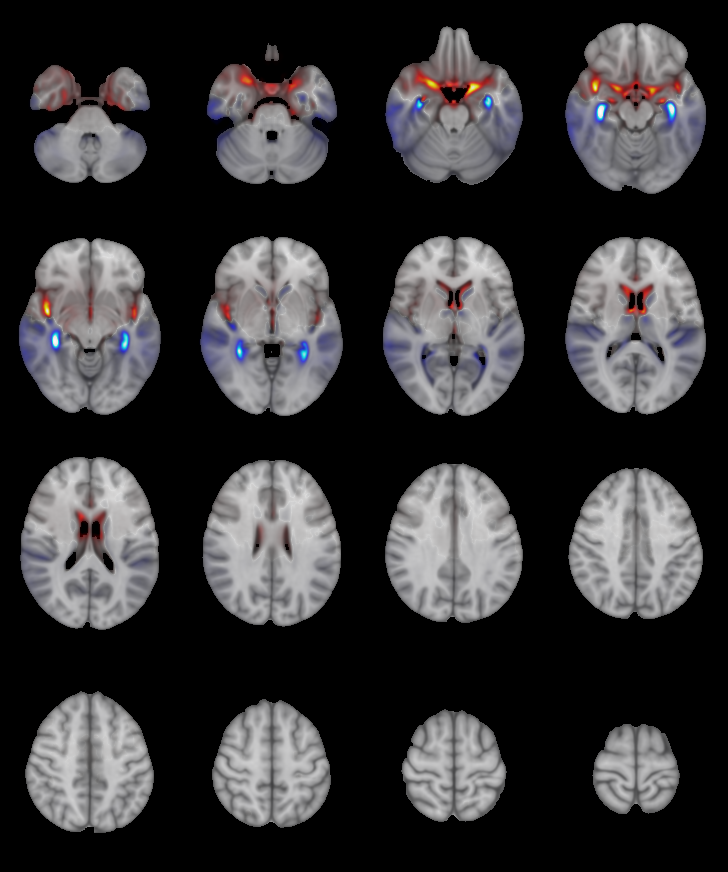
\includegraphics[
                width=\mriwidth,
                clip=true,
                trim = 192mm 232mm 0mm 0mm
            ]{data/components/component_2.png}
        };
        \node[anchor=west] (fourth) at ($ (third.east) + (\gap, 0) $) {
            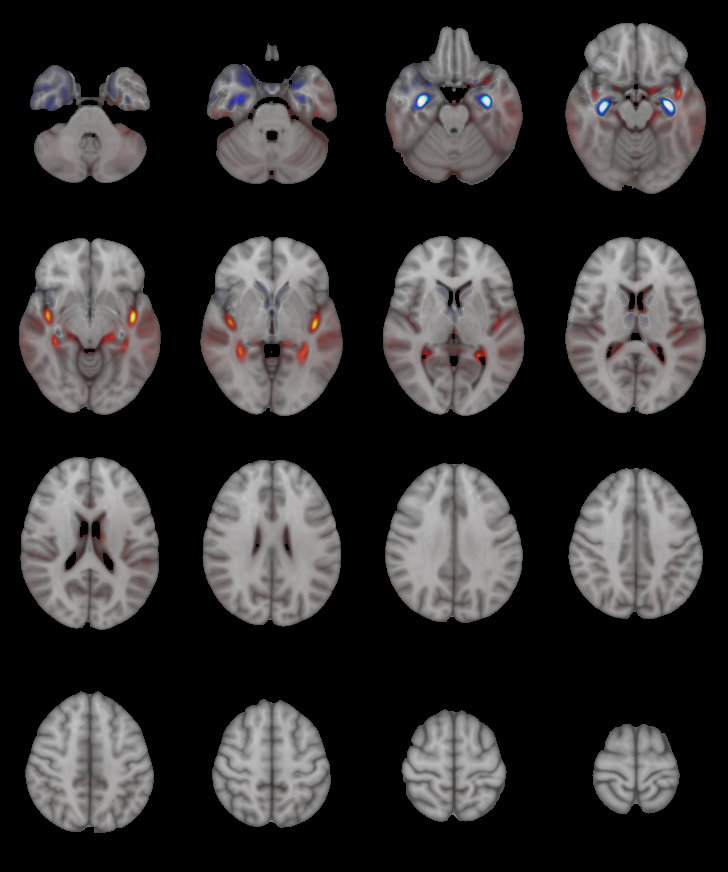
\includegraphics[
                width=\mriwidth,
                clip=true,
                trim = 192mm 232mm 0mm 0mm
            ]{data/components/component_3.png}
        };


        \ifnum#1>0
            \node[anchor=north west] (first-correlation) at ($ (first.south west) + (-0.5, -0.1) $) {
                \hspace{-2.3cm}
                \usebox{\firstcorrelations}
            };
        \fi
        \ifnum#1=2
            \node[anchor=north west] (second-correlation) at ($ (first-correlation.north east) - (0.297, 0) $) {
                \hspace{-2.4cm}
                \usebox{\secondcorrelations}
            };
            \node[anchor=north west] (third-correlation) at ($ (second-correlation.north east) - (0.255, 0) $) {
                \hspace{-2.4cm}
                \usebox{\thirdcorrelations}
            };
            \node[anchor=north west] (fourth-correlation) at ($ (third-correlation.north east) - (0.28, -0.21) $) {
                \hspace{-2.4cm}
                \usebox{\fourthcorrelations}
                \hspace{-0.6cm}
            };
        \fi
    \end{tikzpicture}
}

\newcommand{\prognostic}{
    \begin{tikzpicture}
        \begin{axis}[
            height=3.2cm,
            width=4.1cm,
            xmajorticks=false,
            xmin=0.5,
            xmax=5.5,
            ymin=0.5,
            ymax=1,
            ylabel=\tiny{Accuracy},
            ymajorgrids=true,
            ytick={0.5, 0.6, 0.7, 0.8, 0.9, 1},
            yticklabels={50\%, 60\%, 70\%, 80\%, 90\%, 100\%},
            ytick style={draw=none},
            yticklabel style={font=\tiny, xshift=0.1cm},
            ylabel style={yshift=-0.25cm}
        ]
            \addplot[mark=*, draw=black, mark options={fill=additional}, mark size=2.5pt] coordinates {
                (1, 0.701)
                (2, 0.743)
                (3, 0.771)
                (4, 0.803)
                (5, 0.841)
            };
            \node[anchor=south] at (axis cs: 1, 0.701) {\tiny{70\%}};
            \node[anchor=south] at (axis cs: 2, 0.743) {\tiny{74\%}};
            \node[anchor=south] at (axis cs: 3, 0.771) {\tiny{77\%}};
            \node[anchor=south] at (axis cs: 4, 0.803) {\tiny{80\%}};
            \node[anchor=south] at (axis cs: 5, 0.841) {\tiny{84\%}};
        \end{axis}
    \end{tikzpicture}
}

\newsavebox{\prognosticbox}
\sbox{\prognosticbox}{%
    \prognostic
}

\newcommand{\mciconcept}[1]{
    \begin{tikzpicture}
        \begin{axis}[
            height=0.7\textwidth,
            width=0.8\textwidth,
            xlabel={Age},
            ylabel={Cognitive function},
            ticks=none,
            axis x line=bottom,
            axis y line=left,
            y axis line style={-|},
            xmin=0,
            xmax=1.4,
            ymin=0,
            ymax=1,
            clip=false
        ]
            \addplot[draw=healthy-default, smooth, line width=4pt, opacity=0.5] coordinates {
                (0, 0.9)
                (0.25, 0.87)
                (0.5, 0.77)
                (0.6, 0.72)
                (0.8, 0.63)
                (0.9, 0.72)
                (1.4, 0.67)
            };
            \addplot[draw=controls-default, smooth, line width=4pt, opacity=0.5] coordinates {
                (0, 0.9)
                (0.25, 0.87)
                (0.5, 0.77)
                (0.6, 0.72)
                (0.8, 0.63)
                (0.9, 0.61)
                (1.4, 0.54)
            };
            \addplot[draw=cases-default, smooth, line width=4pt, opacity=0.5] coordinates {
                (0, 0.9)
                (0.25, 0.87)
                (0.5, 0.77)
                (0.6, 0.72)
                (0.8, 0.625)
                (1.1, 0.48)
                (1.4, 0.3)
            };
            \addplot[dashed] coordinates {
                (0, 0.65)
                (1.4, 0.65)
            };
            \addplot[dashed] coordinates {
                (0, 0.4)
                (1.4, 0.4)
            };
            \node[anchor=south west] at (axis cs: 0, 0.64) {\footnotesize{Normal cognition}};
            \node[anchor=north west] at (axis cs: 0, 0.66) {\footnotesize{Mild cognitive impairment}};
            \node[anchor=north west] at (axis cs: 0, 0.41) {\footnotesize{Dementia}};

            \node[anchor=west] at (axis cs: 1.4, 0.67) {\textcolor{healthy-default}{\footnotesize{Improving (n=80)}}};
            \node[anchor=west] at (axis cs: 1.4, 0.53) {\textcolor{controls-default}{\footnotesize{Stable (n=754)}}};
            \node[anchor=west] at (axis cs: 1.4, 0.3) {\textcolor{cases-default}{\footnotesize{Progressive (n=354)}}};

            \ifnum#1>0
                \draw[-stealth, red, thick] (axis cs: 0.8, 0.8) -- (axis cs: 0.8, 0.67);
                \node[anchor=south] at (axis cs: 0.8, 0.8) {\textcolor{red}{\footnotesize{t}}};
            \fi

            \ifnum#1>1
                \draw[densely dotted] (axis cs: 0.9, 0.8) -- (axis cs: 0.9, 0.3);
                \draw[densely dotted] (axis cs: 1, 0.8) -- (axis cs: 1, 0.3);
                \draw[densely dotted] (axis cs: 1.1, 0.8) -- (axis cs: 1.1, 0.3);
                \draw[densely dotted] (axis cs: 1.2, 0.8) -- (axis cs: 1.2, 0.3);
                \draw[densely dotted] (axis cs: 1.3, 0.8) -- (axis cs: 1.3, 0.3);
                \node[anchor=south] at (axis cs: 0.9, 0.8) {\footnotesize{t+1}};
                \node[anchor=south] at (axis cs: 1, 0.8) {\footnotesize{t+2}};
                \node[anchor=south] at (axis cs: 1.1, 0.8) {\footnotesize{t+3}};
                \node[anchor=south] at (axis cs: 1.2, 0.8) {\footnotesize{t+4}};
                \node[anchor=south] at (axis cs: 1.3, 0.8) {\footnotesize{t+5}};
            \fi

            \ifnum#1=3
                \node[] at (axis cs: 1.015, 0.162) {
                    \usebox{\prognosticbox}
                };
            \fi

        \end{axis}
    \end{tikzpicture}
}

\begin{frame}{Explainable AI and dementia}
    \begin{tikzpicture}
        \node[] at (-5.25, -3.5) {};
        \node[] at (5.25, 3.5) {};

        \only<1-2>{
            \node[label={[text depth=0]above:Explainable AI}] at (-2.25, 0) {
				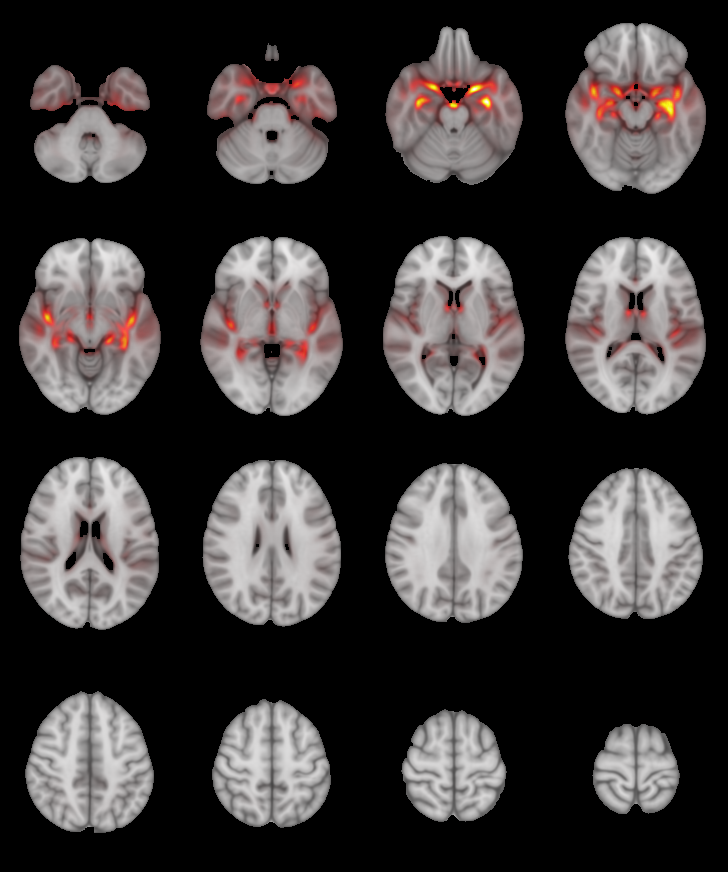
\includegraphics[width=0.31\textwidth]{data/dementia.png}
			};
        }
        \only<2>{
			\node[label={[text depth=0]above:Human researchers}] at (2.25, 0) {
				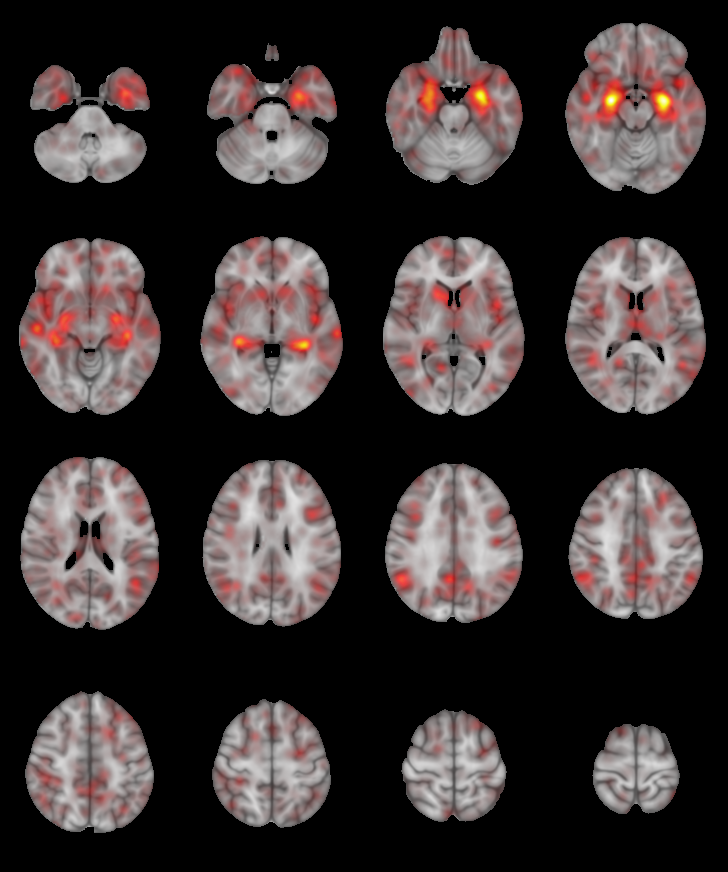
\includegraphics[width=0.31\textwidth]{data/ALE.png}
			};
        }

        \only<3>{
            \node[text width=10cm, font=\scriptsize, align=center] at (0, 0) {
                \renewcommand{\arraystretch}{1.2}
                \begin{tabular}{|>{\centering\arraybackslash}m{2.55cm}|>{\centering\arraybackslash}m{1.45cm}|>{\centering\arraybackslash}m{1.3cm}|>{\centering\arraybackslash}m{2.9cm}|}
                    \hline
                    \textbf{Test battery}&\textbf{Domain}&\textbf{Name}&\textbf{Description}\\
                    \hline
                    Functional Activities Questionnaire&&FAQTOTAL&Measures instrumental activities from everyday life\\
                    \hline
                    ADSP Phenotype Harmonization Consortium&Language&PHC\_LAN&Composite language score\\
                    \hline
                    UW - Neuropsych Summary Scores&Executive functioning&ADNI\_EF&Composite score for executive functioning\\
                    \hline
                    UW - Neuropsych Summary Scores&Memory&ADNI\_MEM&Composite score for memory\\
                    \hline
                \end{tabular}
                \textbf{\vdots}
            };
        }
        \only<4>{
            \node[] at (0.3, 0) {
                \cognitivecorrelations{0}
            };
        }
        \only<5>{
            \node[] at (0.3, 0) {
                \cognitivecorrelations{1}
            };
        }
        \only<6>{
            \node[] at (0.3, 0) {
                \cognitivecorrelations{2}
            };
        }
        \only<7>{
            \node[] at (0, 0) {
                \mciconcept{0}
            };
        }
        \only<8>{
            \node[] at (0, 0) {
                \mciconcept{1}
            };
        }
        \only<9>{
            \node[] at (0, 0) {
                \mciconcept{2}
            };
        }
        \only<10>{
            \node[] at (0, 0) {
                \mciconcept{3}
            };
        }
    \end{tikzpicture}
\end{frame}


    % \begin{frame}{Other conditions}
    %     \begin{tikzpicture}
    %         \node[] at (-5.25, -3.5) {};
    %         \node[] at (5.25, 3.5) {};

    %         \node[] at (0, 0) {
    %             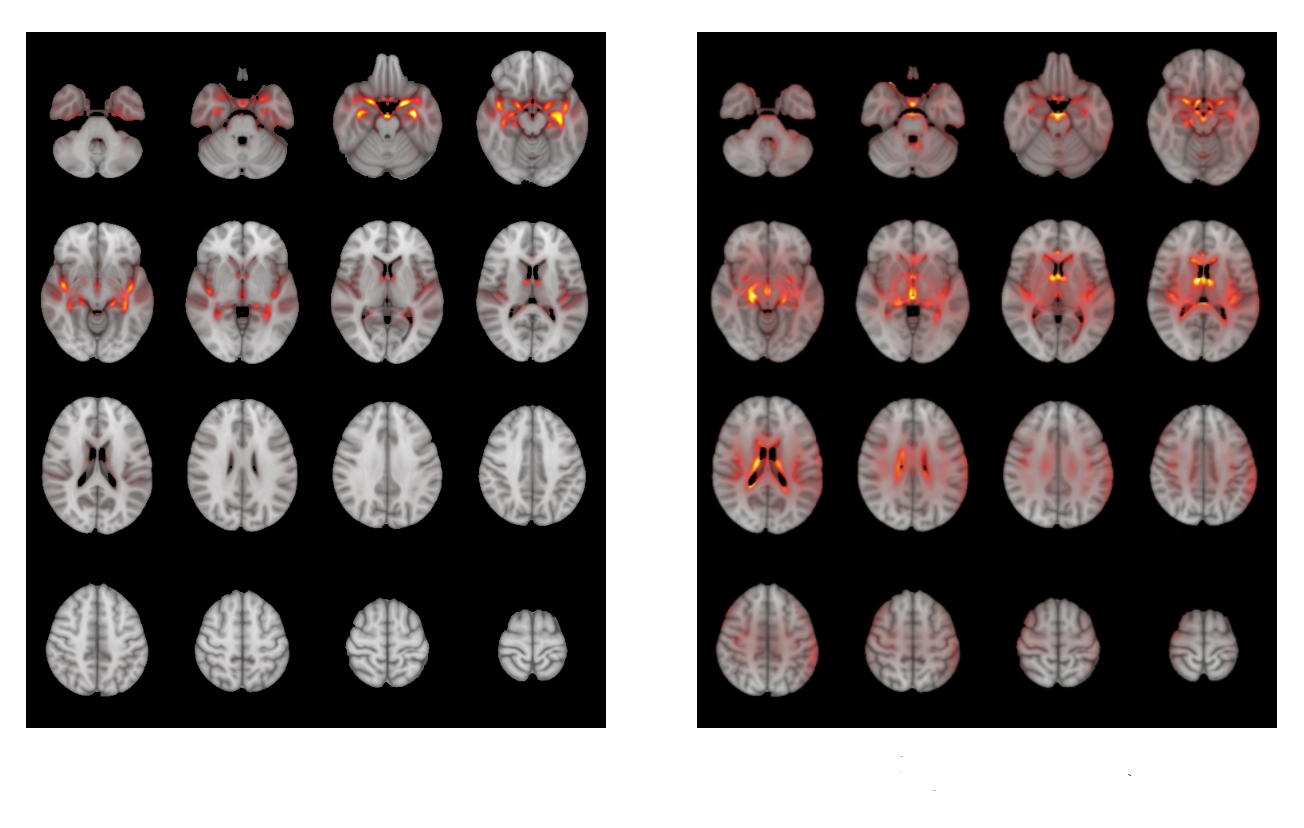
\includegraphics[width=9.5cm]{data/ms.png}
    %         };
    %         \node[] at (-2.45, 3) {
    %             Dementia
    %         };
    %         \node[] at (2.44, 3) {
    %             Multiple sclerosis
    %         };
    %     \end{tikzpicture}
    % \end{frame}
\end{document}
